\documentclass[11pt]{ctexart}
\usepackage[utf8]{inputenc}
\usepackage[left=1in,right=1in,top=1.2in,bottom=1.2in]{geometry}
\usepackage{fancyhdr}
\usepackage{amsmath}
\usepackage{amssymb}
\usepackage{multicol}
\usepackage{ctex}
\usepackage{hyperref}
\usepackage{listings}
\usepackage{xcolor}
\usepackage{graphicx,hyperref,url}
\usepackage{minted}
\usepackage{caption}
\usepackage{subfigure}
\usepackage{listings}
\usepackage{color}

\definecolor{dkgreen}{rgb}{0,0.6,0}
\definecolor{gray}{rgb}{0.5,0.5,0.5}
\definecolor{mauve}{rgb}{0.58,0,0.82}

\usepackage[T1]{fontenc}
\usepackage{mathpazo}
\usepackage{fontspec}
\setmainfont{TeX Gyre Pagella}
\setCJKmainfont[ItalicFont=Noto Sans CJK SC Bold, BoldFont=Noto Serif CJK SC Black]
{Noto Serif CJK SC}

\lstset{frame=tb,
  language=Python,
  aboveskip=3mm,
  belowskip=3mm,
  showstringspaces=false,
  columns=flexible,
  basicstyle={\small\ttfamily},
  numbers=none,
  numberstyle=\tiny\color{gray},
  keywordstyle=\color{blue},
  commentstyle=\color{dkgreen},
  stringstyle=\color{mauve},
  breaklines=true,
  breakatwhitespace=true,
  tabsize=3
}

% \usepackage{titlesec}
% \titlespacing\section{0pt}{15pt}{0pt}
% \titlespacing\subsection{0pt}{5pt}{0pt}
% \titlespacing\subsubsection{0pt}{5pt}{0pt}

\usepackage{enumitem}
\setlist{nolistsep}

\pagestyle{fancy}
\fancyhead[L]{East China Normal University}
\fancyhead[R]{\thepage}
\fancyfoot[C]{}

\fancypagestyle{plain}
{
\fancyhead[L]{East China Normal University}
\fancyhead[R]{\thepage}
\fancyfoot[C]{}
}

\ctexset{section/format=\Large\bfseries}



\setcounter{page}{1}

\title{华东师范大学软件工程实验报告}
\author{谢嘉东\ 10185101247\\陈俊潼\ 10185101210}
\date{May 2020}

\begin{document}

\maketitle

\thispagestyle{empty}

\begin{itemize}
    \item 课程名称:数字图像处理
    \item 年级:2018 级本科
    \item 实验编号:实验 004
    \item 上机实践日期:2020.5
\end{itemize}

\tableofcontents

\thispagestyle{empty}

\newpage

\section{分工情况}

组内两人共同查阅资料,完善代码,完成了实验部分和附加题。

实验报告由两人共同撰写。

\section{实验内容}

图像锐化(image sharpening)与图像平滑是作用相反的操作。它是通过加强图像的轮廓,增强图像的边缘及灰度跳变的部分,使图像变得清晰,常用方法有微分法、高通滤波法和反锐化掩模法。

形态学,即数学形态学(Mathematical Morphology),在图像处理中的主要应用是提取·图像中对于表达和描绘区域形状有意义的图像分量,使后续的识别工作能够抓住目标对象最为本质的形状特征,像素边界和连通区域等。二值图像的基本形态学运算包括腐蚀、膨胀、开操作和闭操作。
图像变换包括伪彩色处理、代数运算和几何变换三部分。

几何变换(geometric transformation)包括平移、旋转、放缩、反转、前/后向映射、线性内插等等,几何变换不改变像素值,而是改变像素所在的位置。

本次实验中我们通过 Python 和 OpenCV 库实现了图像锐化、形态学处理和图像的几何变换,包括仿射变换、相似变换、欧拉变换、刚体变换等。

\section{实验目的}

\begin{itemize}
    \item [1] 了解 Python OpenCV 库对图像的基本操作
    \item [2] 掌握图像锐化的原理和实现方法
    \item [3] 实现图像的形态学处理,了解腐蚀、膨胀、开操作、闭操作等形态学处理方法的原理
    \item [4] 实现图像的几何变换
\end{itemize}

\section{实验原理}

利用 numpy 、matplotlib.pyplot 、cv2 、imageio 、skimage 以及 Pillow 中的 PIL 包来辅助完成实验。其中主要用到了:

\begin{itemize}
    \item cv.erode(src, dst, element=None, iterations=1)
    \begin{itemize}
        \item src – input image; the number of channels can be arbitrary, but the depth should be one of CV\_8U, CV\_16U, CV\_16S, CV\_32F` or ``CV\_64F.
        \item dst – output image of the same size and type as src.
        \item element – structuring element used for erosion; if element=Mat() , a 3 x 3 rectangular structuring element is used.
        \item anchor – position of the anchor within the element; default value (-1, -1) means that the anchor is at the element center.
        \item iterations – number of times erosion is applied.
        \item borderType – pixel extrapolation method
        \item borderValue – border value in case of a constant border
    \end{itemize}
\end{itemize}


\begin{itemize}
    \item cv.dilate(src, dst, element=None, iterations=1)
     \begin{itemize}
    \item src – input image; the number of channels can be arbitrary, but the \item depth should be one of CV\_8U, CV\_16U, CV\_16S, CV\_32F` or ``CV\_64F.
    \item dst – output image of the same size and type as src.
    \item element – structuring element used for dilation; if element=Mat() , a 3 x 3 rectangular structuring element is used.
    \item anchor – position of the anchor within the element; default value (-1, -1) means that the anchor is at the element center.
    \item iterations – number of times dilation is applied.
    \item borderType – pixel extrapolation method
    \item borderValue – border value in case of a constant border
    \end{itemize}
\end{itemize}



    \begin{itemize}
        \item
          \texttt{cv.GetRotationMatrix2D}(center, angle, scale, mapMatrix)
          \begin{itemize}
          \item
            \textbf{center} -- Center of the rotation in the source image.
          \item
            \textbf{angle} -- Rotation angle in degrees. Positive values mean
            counter-clockwise rotation (the coordinate origin is assumed to be
            the top-left corner).
          \item
            \textbf{scale} -- Isotropic scale factor.
          \item
            \textbf{map\_matrix} -- The output affine transformation, 2x3
            floating-point matrix.
          \end{itemize}
    \end{itemize}


    \begin{itemize}
    \item
      \texttt{cv.WarpAffine}(src, dst, mapMatrix,
      flags=CV\emph{INTER}LINEAR+CV\emph{WARP}FILL\_OUTLIERS, fillval=(0, 0,
      0, 0))
      \begin{itemize}
      \item
        \textbf{src} -- input image.
      \item
        \textbf{dst} -- output image that has the size \texttt{dsize} and
        the same type as \texttt{src} .
      \item
        \textbf{M} -- \(2 \times 3\) transformation matrix.
      \item
        \textbf{dsize} -- size of the output image.
      \item
        \textbf{flags} -- combination of interpolation methods
      \item
        \textbf{borderMode} -- pixel extrapolation method
      \item
        \textbf{borderValue} -- value used in case of a constant border; by
        default, it is 0.
        \end{itemize}
    \end{itemize}

    \begin{itemize}
    \item numpy.array(object, dtype=None, copy=True, order='K', subok=False, ndmin=0)
    \begin{itemize}
        \item object : array\_like
        \item dtype : data-type, optional
        \item copy : bool, optional
        \item order : {‘K’, ‘A’, ‘C’, ‘F’}, optional
        \item subok : bool, optional
        \item ndmin : int, optional
    \end{itemize}

    \item scipy.ndimage.filters.gaussian\_filter(input, sigma, order=0, output=None, mode='reflect', cval=0.0, truncate=4.0)
    \begin{itemize}
        \item input : array\_like, Input array to filter.
        \item sigma : scalar or sequence of scalars
    \end{itemize}


   \item scipy.ndimage.filters.minimum\_filter(input, sigma, order=0, output=None, mode='reflect', cval=0.0, truncate=4.0)
    \begin{itemize}
        \item input : array\_like, Input array to filter.
        \item sigma : scalar or sequence of scalars
    \end{itemize}

\item scipy.ndimage.filters.maximum\_filter(input, sigma, order=0, output=None, mode='reflect', cval=0.0, truncate=4.0)
    \begin{itemize}
        \item input : array\_like, Input array to filter.
        \item sigma : scalar or sequence of scalars
    \end{itemize}
\end{itemize}

\section{实验方法}

\subsection{反锐化掩膜}

反锐化掩模技术最早应用于摄影技术中,以增强图像的边缘和细节。光学上的操作方法是将聚焦的正片和散焦的负片在底片上进行叠加,结果是增强了正片高频成份,从而增强了轮廓,散焦的负片相当于“模糊”模板(掩模),与锐化的作用正好相反。其原理可如图 \ref{um} 所示:

\begin{figure}[htbp]
    \centering
    \includegraphics[width=0.6\textwidth]{um.jpg}
    \caption{反锐化掩膜原理}
    \label{um}
\end{figure}

对原图 $G$ 使用高斯模糊,得到经过低通滤波的图像 $G'$,设强化率为 $\alpha$,则经过反锐化掩膜得到的图像为 $G + \alpha (G - G')$。

\subsection{形态学处理}

膨胀和腐蚀是形态学图像处理的两个基本运算,膨胀可以使图像扩大(如字体图像加粗);腐蚀可以使图像缩小(如消除图像中不重要的细节部分).

\paragraph{膨胀} 使用结构形态元 B 处理图像 A,膨胀的计算公式为:

$$
A \oplus B = \{z | (\hat{(B)}_z \cap A \ne \emptyset ) \}
$$

预先定义好结构元,可以使用 \texttt{opencv.dilate} 实现该运算。

\paragraph{腐蚀} 使用结构形态元 B 处理图像 A,腐蚀的计算公式为:

$$
A \ominus B = \{z | (B)_z \subseteq A \}
$$

可以使用 \texttt{opencv.erode} 实现该功能。


\subsection{几何变换}

几何变换不改变像素的值,而只改变像素所在的位置。使用放射矩阵可以对图像进行几何变换。通常使用一个 $2 \times 3$ 的矩阵来实现各种放射变换。其形式如下:

$$
A = \begin{bmatrix} a_{00} & a_{01} \\ a_{10} & a_{11} \end{bmatrix}_{2 \times 2}
B = \begin{bmatrix} b_{00} \\ b_{10} \end{bmatrix}_{2 \times 1} \\ \newline
M = \begin{bmatrix} A & B \end{bmatrix} = \begin{bmatrix} a_{00} & a_{01} & b_{00} \\ a_{10} & a_{11} & b_{10} \end{bmatrix}_{2 \times 3}
$$

利用变换矩阵 M,对于任何一个像素 $X = \begin{bmatrix}x \\ y\end{bmatrix}$,有:

$$
T = A \cdot \begin{bmatrix}x \\ y\end{bmatrix} + B = M \cdot [x, y, 1]^{T}
$$

特别地,对于旋转操作,有:

$$
M = \begin{bmatrix}
\cos \theta & \sin \theta & 0 \\
-\sin \theta & \cos \theta & 0
\end{bmatrix}
$$

通过 \texttt{cv2.getAffineTransform} 可以根据三个瞄点得到对应的变换矩阵。通过 \texttt{cv2.warpAffine} 可以实现各种放射变换。

\subsection{胸透 X 光图片锐化及增强}

通过查阅相关文献以及经过长时间的调整参数,我们最终利用 Unsharp Masking 技术得到了效果较好的图像结果。

Unsharp Masking 是一种线性滤波器,能够放大图像的高频。这个算法的有点在于,运行的效率十分高,时间复杂度是 $O(n)$ ,可以在比较短的时间内给出处理结果,且效果较好。

算法首先需要复制原始图像,并在其中应用 Gaussian Blur (模糊强度的设置定义为参数 \texttt{radius} )。如果从原始图像中减去模糊的图像,我们将仅获得由模糊创建的边缘。

最后,通过查阅文献中的方法,应用以下公式收集增强后的图像:

\texttt{sharpened image = original image + amount * (unsharped mask)}

可惜的是,\texttt{amount} 以及 \texttt{radius} 没有很好的方法来确定他们,所以我们在实验的过程中,只能通过不断的调节这两个参数来获取相对理想的结果。

同时,通过阅读 \texttt{scipy.ndimage.filters} 的文档,得知除了 Gaussian Blur 外,还有 Minimum Blur 和 Maximum Blur,于是我们也同样利用这两个蒙板技术来对比之前的处理,发现他们在不同的图像情况下,会得到不同的效果,而无法确切断定谁的效果更加理想,可能需要根据具体的应用场景来决定。

三个过滤器效果的比较会在下一节给出,在这里仅对于\texttt{amount} 以及 \texttt{radius}大小的调整过程进行比较(以 胸透X.jpg 为例)。

   \begin{figure}[htbp]
        \centering
        \subfigure[\texttt{radius} $=1$]{
            \begin{minipage}[t]{0.4\linewidth}
            \centering
            \includegraphics[width=0.6\textwidth]{output/胸透X_output_0.jpg}
        \end{minipage}
        }
        \subfigure[\texttt{radius} $=5$]{
            \begin{minipage}[t]{0.4\linewidth}
            \centering
            \includegraphics[width=0.6\textwidth]{output/胸透X_output_5.jpg}
            \end{minipage}
        }
        \subfigure[\texttt{radius} $=10$]{
            \begin{minipage}[t]{0.4\linewidth}
            \centering
            \includegraphics[width=0.6\textwidth]{output/胸透X_output_10.jpg}
        \end{minipage}
        }
        \subfigure[\texttt{radius} $=20$]{
            \begin{minipage}[t]{0.4\linewidth}
            \centering
            \includegraphics[width=0.6\textwidth]{output/胸透X_output_20.jpg}
            \end{minipage}
        }
        \centering
        \caption{模糊强度大小设置比较}\label{fig:digit}
  \end{figure}

\newpage

从肉眼观察的角度来说,\texttt{radius} $=5$ 的时候效果相对比较理想,所以我们最终的实验效果图选择了 \texttt{radius} $=5$ 的结果。

接下来,我们比较了不同的 \texttt{amount} 取值会对图像收集增强产生的不同效果。

   \begin{figure}[htbp]
        \centering
        \subfigure[\texttt{amount} $=1$]{
            \begin{minipage}[t]{0.4\linewidth}
            \centering
            \includegraphics[width=0.6\textwidth]{output/胸透X_output_rad_0.jpg}
        \end{minipage}
        }
        \subfigure[\texttt{amount} $=2$]{
            \begin{minipage}[t]{0.4\linewidth}
            \centering
            \includegraphics[width=0.6\textwidth]{output/胸透X_output_rad_2.jpg}
            \end{minipage}
        }
        \subfigure[\texttt{amount} $=5$]{
            \begin{minipage}[t]{0.4\linewidth}
            \centering
            \includegraphics[width=0.6\textwidth]{output/胸透X_output_rad_5.jpg}
        \end{minipage}
        }
        \subfigure[\texttt{amount} $=10$]{
            \begin{minipage}[t]{0.4\linewidth}
            \centering
            \includegraphics[width=0.6\textwidth]{output/胸透X_output_rad_10.jpg}
            \end{minipage}
        }
        \centering
        \caption{\texttt{amount} 大小设置比较}\label{fig:digit}
  \end{figure}

根据效果的对比,我们最终选择了 \texttt{amount} $=2$ 最为我们的最终效果图。


\section{实验结果及分析}

基本完成了实验预期所要达到的要求。

最终的实验结果如下:

\subsection*{反锐化掩膜}

    \begin{figure}[htbp]
        \centering
        \subfigure[原图]{
            \begin{minipage}[t]{0.4\linewidth}
            \centering
            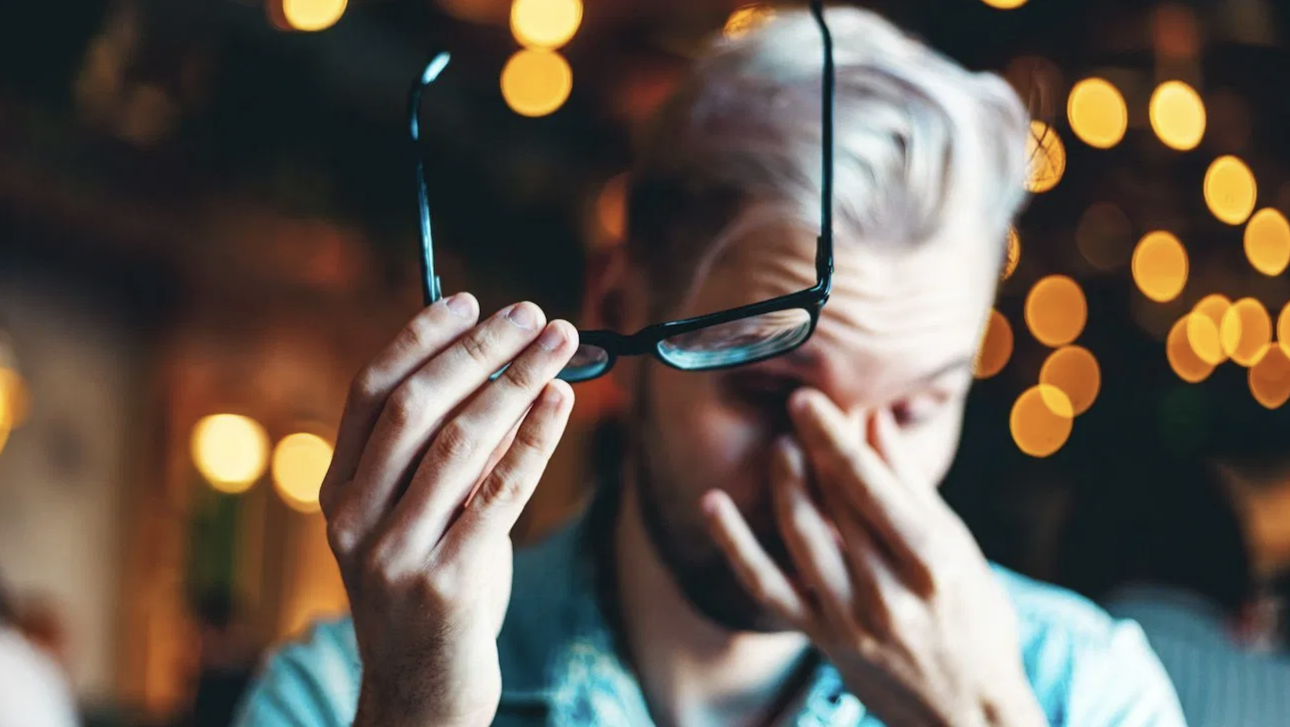
\includegraphics[width=0.9\textwidth]{input/1.3.png}
        \end{minipage}
        }
        \subfigure[结果]{
            \begin{minipage}[t]{0.4\linewidth}
            \centering
            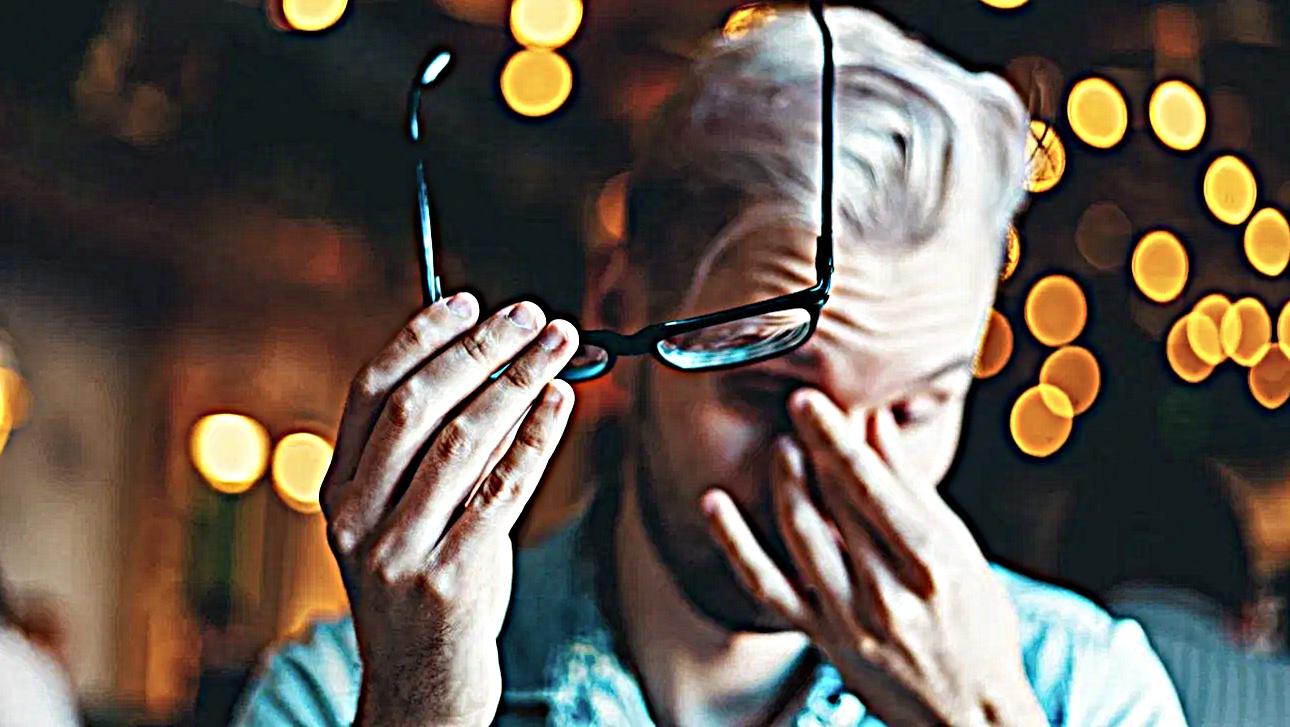
\includegraphics[width=0.9\textwidth]{output/1.3.jpg}
            \end{minipage}
        }
        \subfigure[原图]{
            \begin{minipage}[t]{0.4\linewidth}
            \centering
            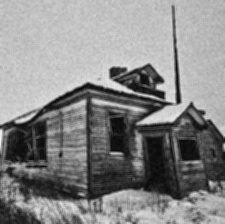
\includegraphics[width=0.9\textwidth]{input/1.3_1.jpg}
        \end{minipage}
        }
        \subfigure[结果]{
            \begin{minipage}[t]{0.4\linewidth}
            \centering
            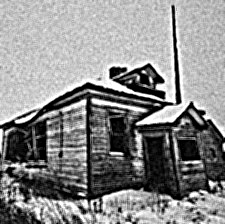
\includegraphics[width=0.9\textwidth]{output/1.3_1.jpg}
            \end{minipage}
        }
        \centering
        \caption{反锐化掩膜}\label{fig:digit}
  \end{figure}

\newpage

\subsection* {形态学处理}

   \begin{figure}[htbp]
        \centering
        \subfigure[原图]{
            \begin{minipage}[t]{0.4\linewidth}
            \centering
            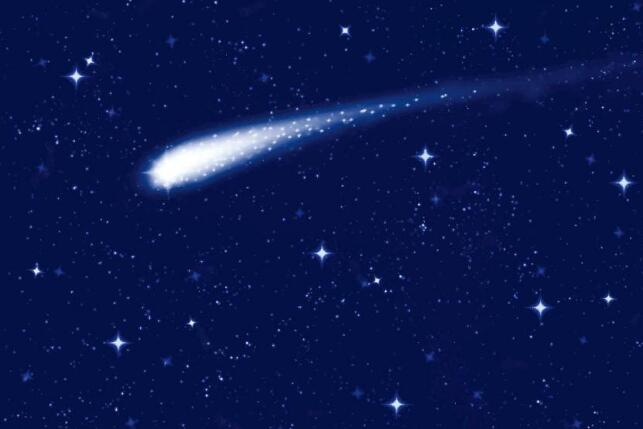
\includegraphics[width=0.6\textwidth]{input/2.1_1.jpg}
        \end{minipage}
        }
        \subfigure[结果]{
            \begin{minipage}[t]{0.4\linewidth}
            \centering
            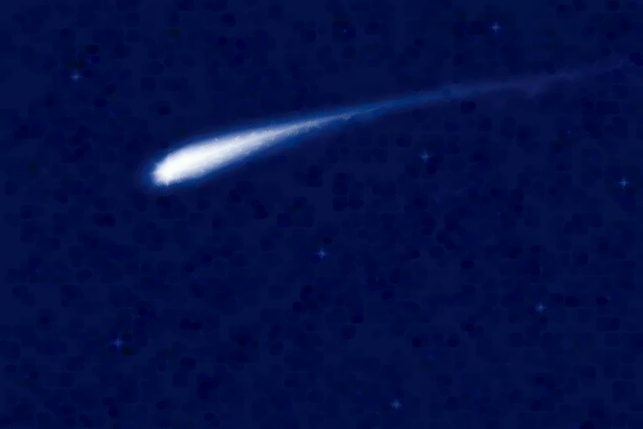
\includegraphics[width=0.6\textwidth]{output/2.1_1.jpg}
            \end{minipage}
        }
        \subfigure[原图]{
            \begin{minipage}[t]{0.4\linewidth}
            \centering
            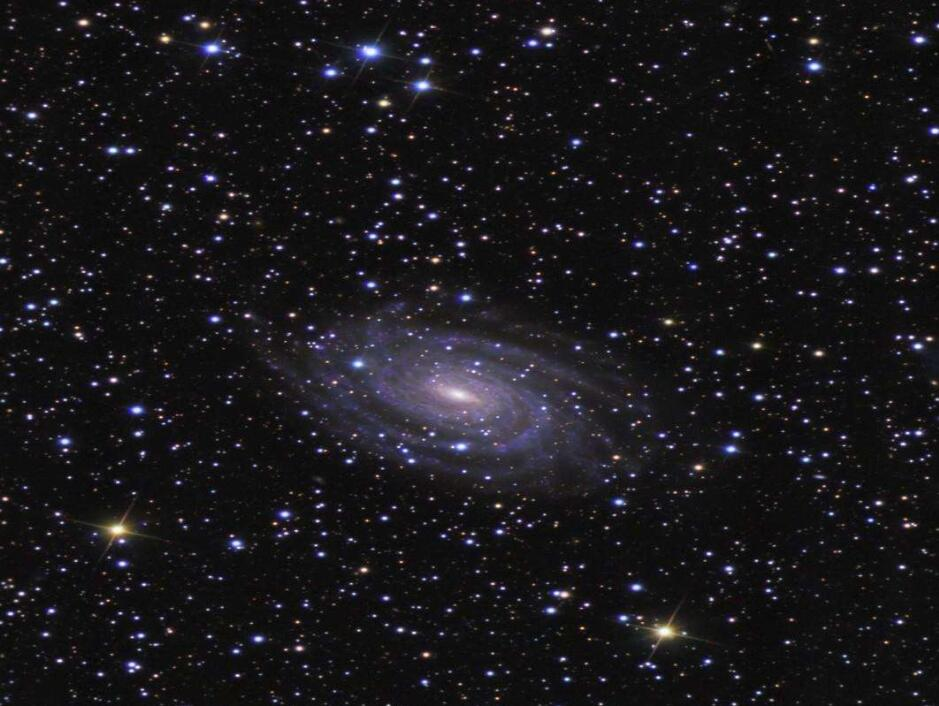
\includegraphics[width=0.6\textwidth]{input/2.1_2.jpg}
        \end{minipage}
        }
        \subfigure[结果]{
            \begin{minipage}[t]{0.4\linewidth}
            \centering
            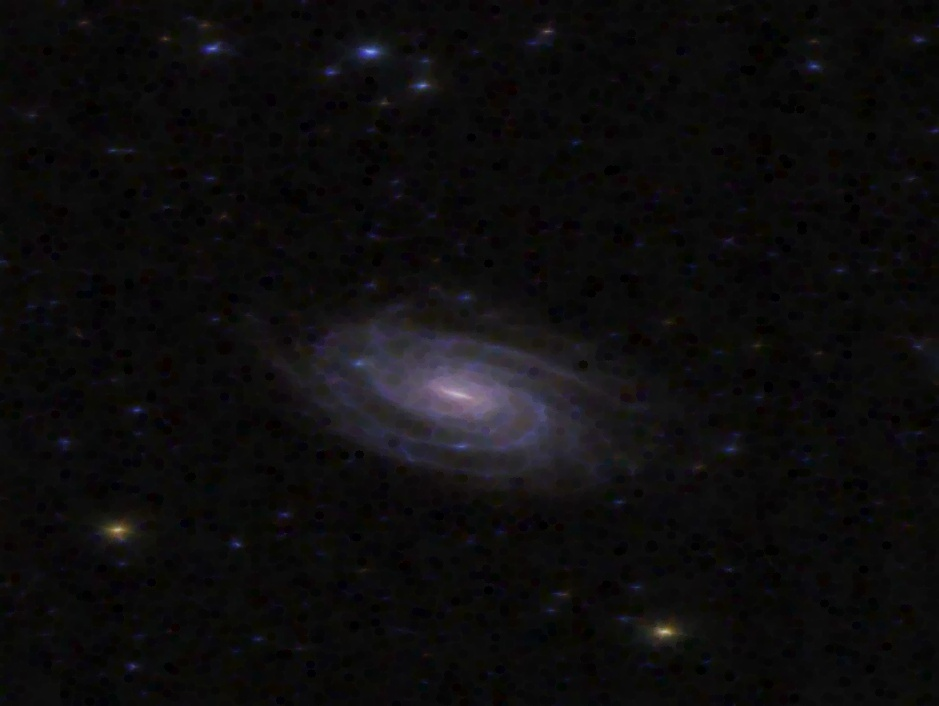
\includegraphics[width=0.6\textwidth]{output/2.1_2.jpg}
            \end{minipage}
        }
        \centering
        \caption{腐蚀}\label{fig:digit}
  \end{figure}


 \begin{figure}[htbp]
    \centering
    \subfigure[原图]{
        \begin{minipage}[t]{0.4\linewidth}
        \centering
        
\includegraphics[width=0.5\textwidth]{input/2.1_3.jpg}
    \end{minipage}
    }
    \subfigure[结果]{
        \begin{minipage}[t]{0.4\linewidth}
        \centering
        
\includegraphics[width=0.5\textwidth]{output/2.1_3.jpg}
        \end{minipage}
    }
    \subfigure[原图]{
        \begin{minipage}[t]{0.4\linewidth}
        \centering
        
\includegraphics[width=0.5\textwidth]{input/2.1_4.jpg}
    \end{minipage}
    }
    \subfigure[结果]{
        \begin{minipage}[t]{0.4\linewidth}
        \centering
        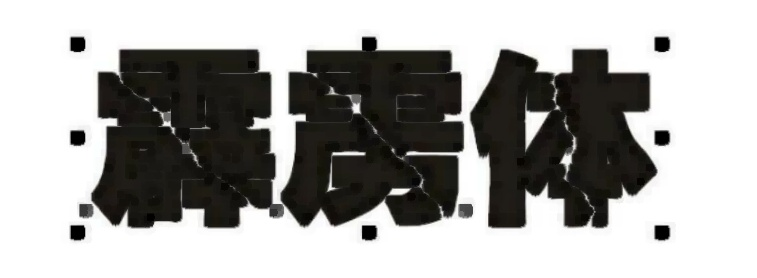
\includegraphics[width=0.5\textwidth]{output/2.1_4.jpg}
        \end{minipage}
    }
    \centering
    \caption{膨胀(膨胀前经反色处理)}\label{fig:digit}
\end{figure}

\newpage

\subsection*{几何变换}


\begin{figure}[htbp]
    \centering
    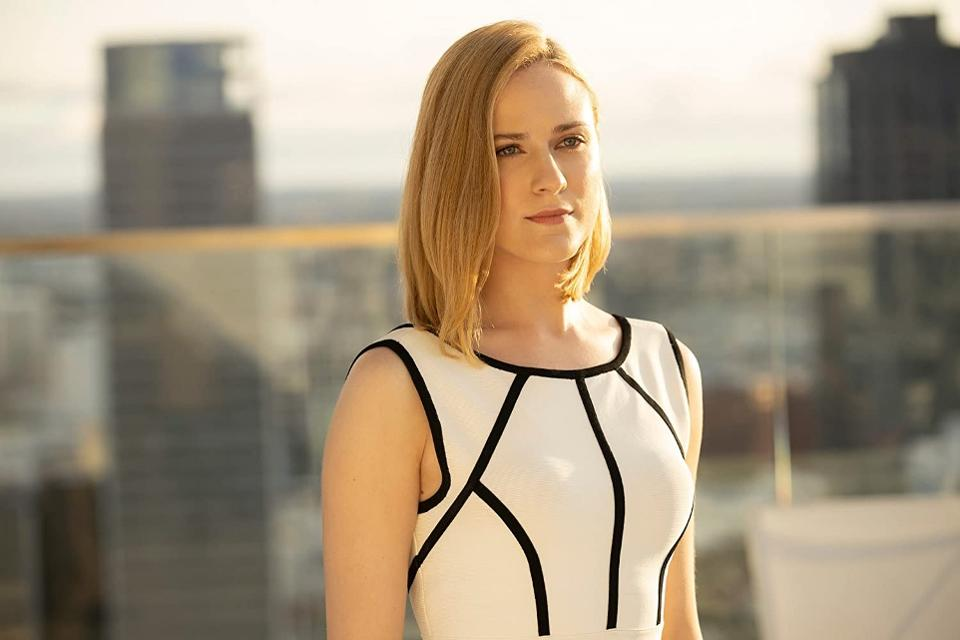
\includegraphics[width=0.4\textwidth]{input/3.3.jpg}
    \caption{几何变换原图}
\end{figure}

 \begin{figure}[htbp]
    \centering
    \subfigure[仿射变换]{
        \begin{minipage}[t]{0.4\linewidth}
        \centering
        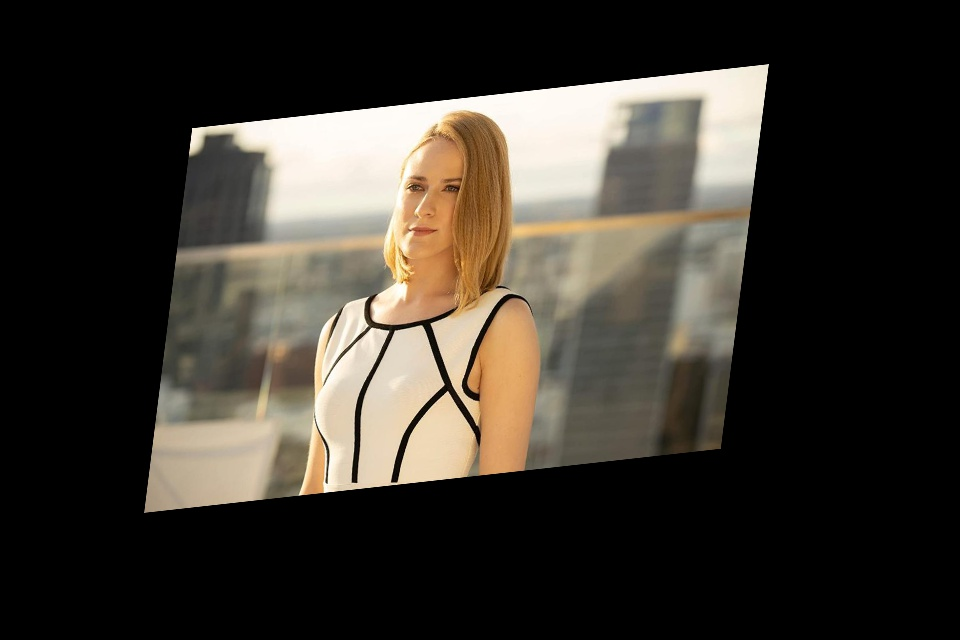
\includegraphics[width=0.8\textwidth]{output/3.3_affine.jpg}
        \end{minipage}
    }
    \subfigure[相似变换]{
        \begin{minipage}[t]{0.4\linewidth}
        \centering
        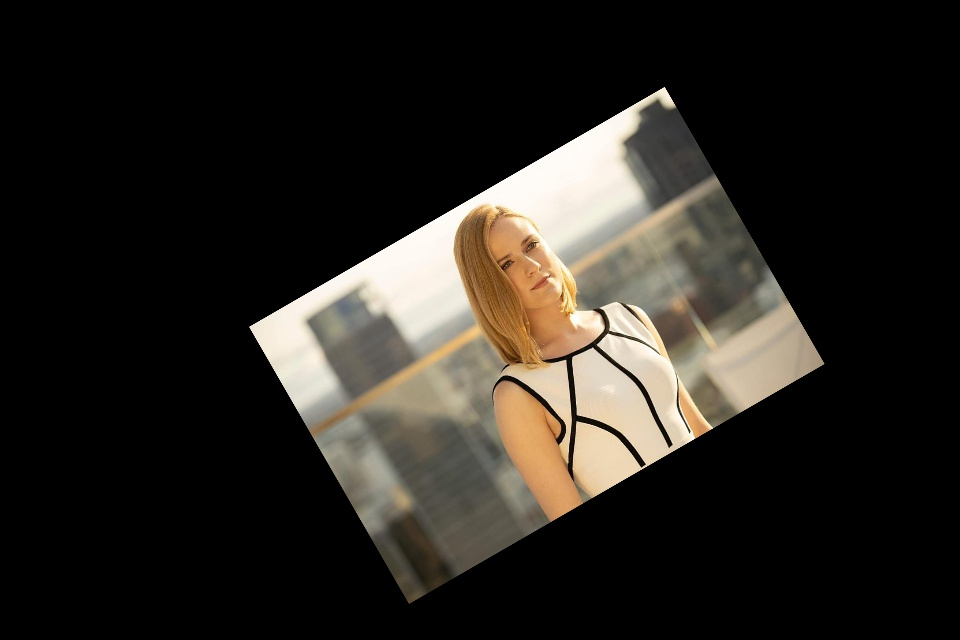
\includegraphics[width=0.8\textwidth]{output/3.3_similarity.jpg}
    \end{minipage}
    }
    \subfigure[刚体变换]{
        \begin{minipage}[t]{0.4\linewidth}
        \centering
        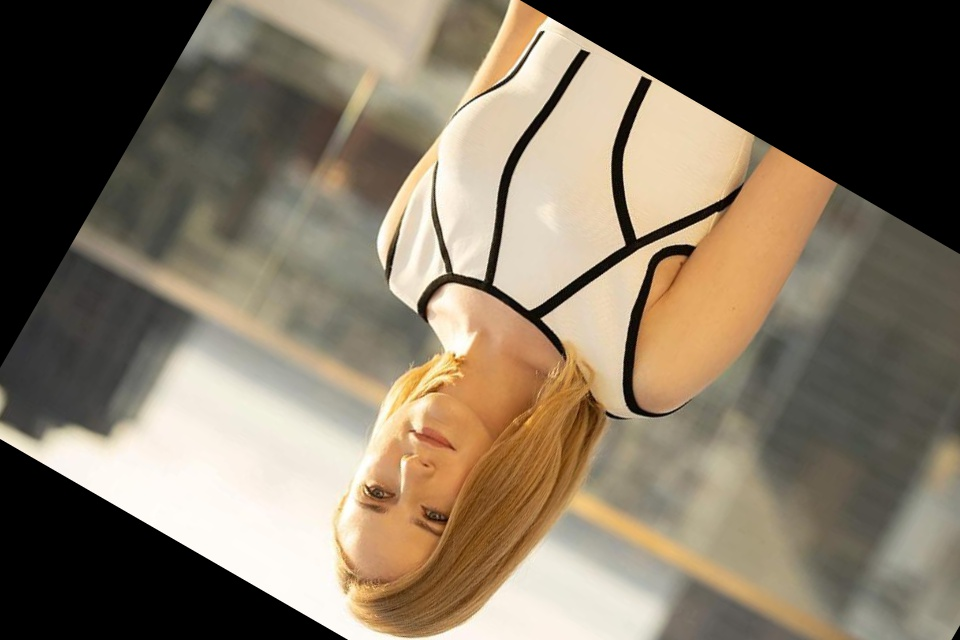
\includegraphics[width=0.8\textwidth]{output/3.3_rigid_body.jpg}
    \end{minipage}
    }
    \subfigure[欧拉变换]{
        \begin{minipage}[t]{0.4\linewidth}
        \centering
        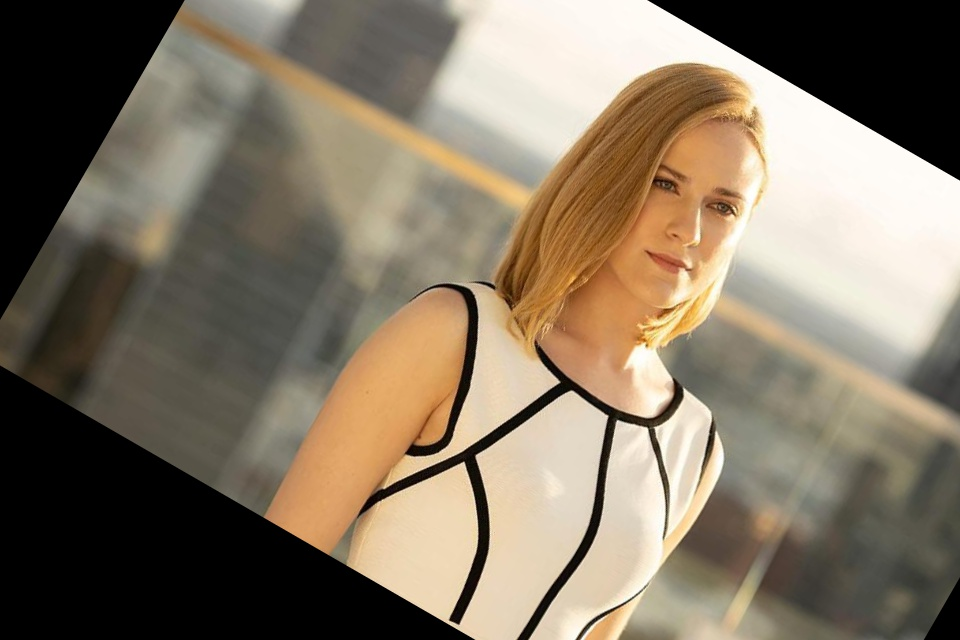
\includegraphics[width=0.8\textwidth]{output/3.3_eular.jpg}
        \end{minipage}
    }
    \centering
    \caption{几何变换处理结果}\label{fig:digit}
  \end{figure}

\newpage

\subsection*{胸透 X 光图片锐化及增强}


   \begin{figure}[htbp]
    \centering
    \subfigure[原图]{
        \begin{minipage}[t]{0.4\linewidth}
        \centering
        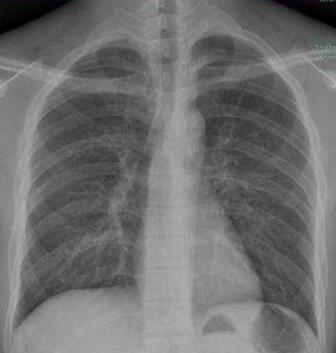
\includegraphics[width=0.8\textwidth]{input/胸透X2.jpg}
        \end{minipage}
    }
    \subfigure[gaussian\_filter]{
        \begin{minipage}[t]{0.4\linewidth}
        \centering
        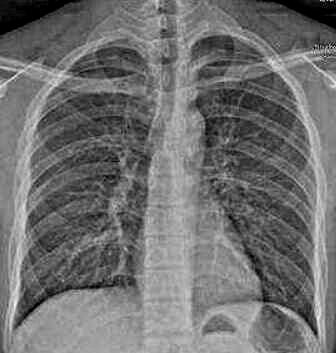
\includegraphics[width=0.8\textwidth]{output/胸透X2_output_1.jpg}
    \end{minipage}
    }
    \subfigure[minimum\_filter]{
        \begin{minipage}[t]{0.4\linewidth}
        \centering
        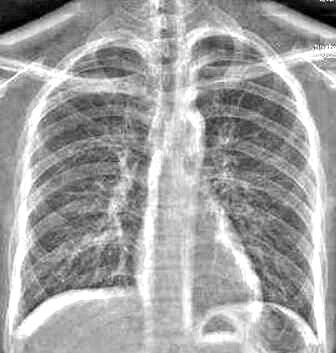
\includegraphics[width=0.8\textwidth]{output/胸透X2_output_2.jpg}
    \end{minipage}
    }
    \subfigure[maximum\_filter]{
        \begin{minipage}[t]{0.4\linewidth}
        \centering
        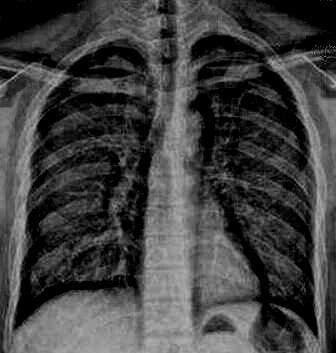
\includegraphics[width=0.8\textwidth]{output/胸透X2_output_3.jpg}
        \end{minipage}
    }
    \centering
    \caption{胸透X光图片处理结果}\label{fig:digit}
  \end{figure}

\newpage

 \begin{figure}[htbp]
    \centering
    \subfigure[原图]{
        \begin{minipage}[t]{0.4\linewidth}
        \centering
        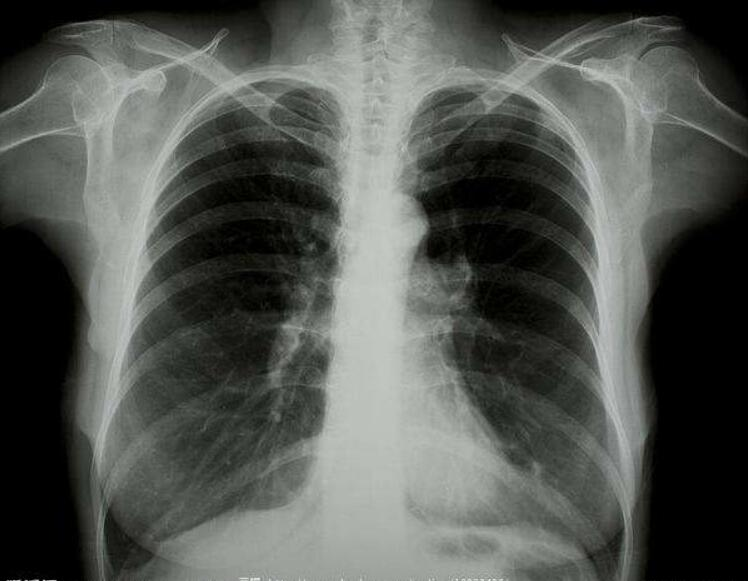
\includegraphics[width=0.8\textwidth]{input/胸透X.jpg}
        \end{minipage}
    }
    \subfigure[gaussian\_filter]{
        \begin{minipage}[t]{0.4\linewidth}
        \centering
        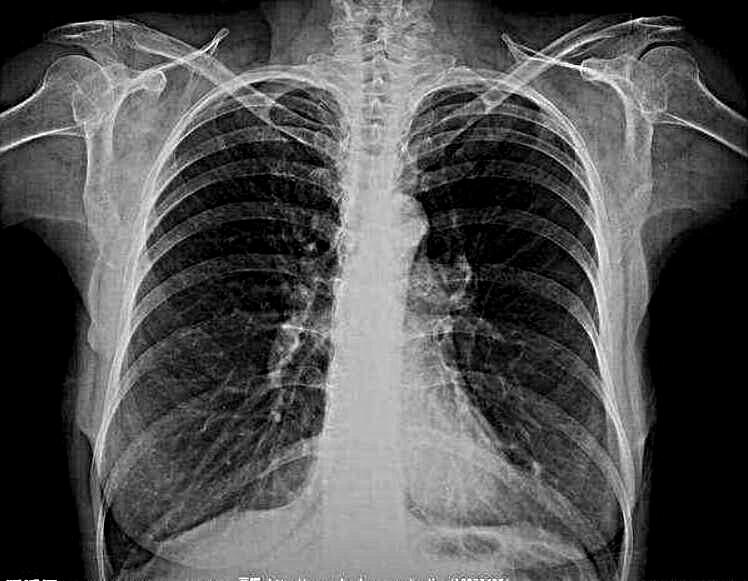
\includegraphics[width=0.8\textwidth]{output/胸透X_output_1.jpg}
    \end{minipage}
    }
    \subfigure[minimum\_filter]{
        \begin{minipage}[t]{0.4\linewidth}
        \centering
        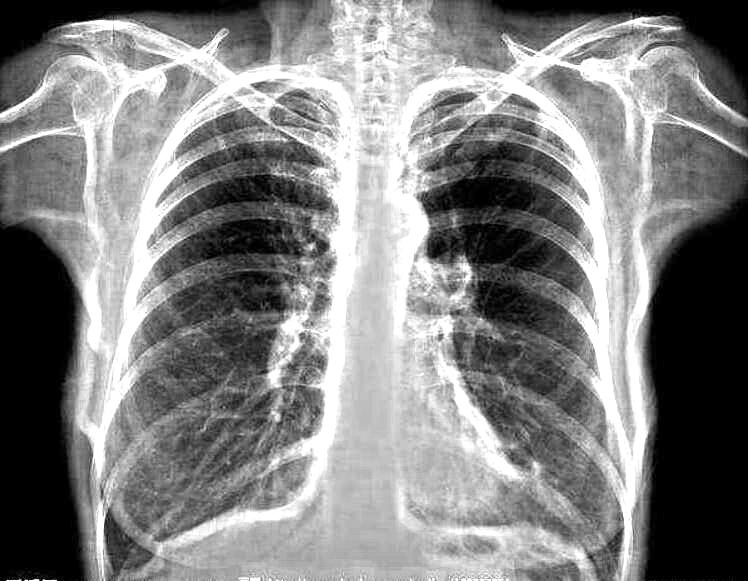
\includegraphics[width=0.8\textwidth]{output/胸透X_output_2.jpg}
    \end{minipage}
    }
    \subfigure[maximum\_filter]{
        \begin{minipage}[t]{0.4\linewidth}
        \centering
        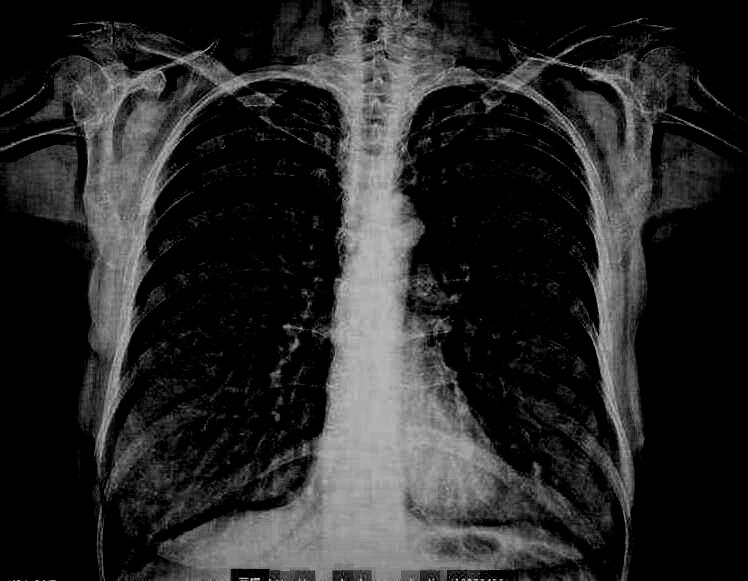
\includegraphics[width=0.8\textwidth]{output/胸透X_output_3.jpg}
        \end{minipage}
    }
    \centering
    \caption{胸透X光图片处理结果2}\label{fig:digit}
  \end{figure}

\section{主要核心代码}

\paragraph{反锐化掩膜}

\lstset{language=python}
\begin{lstlisting}
import cv2
import numpy as np
import matplotlib.pyplot as plt

def unsharp_masking(input, ratio = 1.0, ksize = 9):
	"""Return a sharpened version of the image, using an unsharp mask."""
	blurred = cv2.GaussianBlur(input, (ksize, ksize), 0)
	# 锐化后的图像 = 原图像 + ratio * (原图像 - 模糊图像)
	sharpened = float(1 + ratio) * input- ratio * blurred
	# 限制值在 0 - 255 之间
	sharpened = np.maximum(sharpened, np.zeros(sharpened.shape))
	sharpened = np.minimum(sharpened, 255 * np.ones(sharpened.shape))
	sharpened = sharpened.round().astype(np.uint8)
	return sharpened

img = cv2.imread('input/1.3.png')
output = unsharp_masking(img, 1.8, 35)
cv2.imwrite('output/1.3.jpg', output, [int(cv2.IMWRITE_JPEG_QUALITY), 95])

img = cv2.imread('input/1.3_1.jpg')
output = unsharp_masking(img, 1.8, 35)
cv2.imwrite('output/1.3_1.jpg', output, [int(cv2.IMWRITE_JPEG_QUALITY), 95])

\end{lstlisting}

\paragraph{形态学变换}

\lstset{language=python}
\begin{lstlisting}
import cv2
import numpy as np
import matplotlib.pyplot as plt

def dilation(img, ksize = 9):
	"""Dilation of an image."""
	kernel = cv2.getStructuringElement(cv2.MORPH_ELLIPSE, (ksize, ksize))
	dialation = cv2.dilate(img, kernel)
	return dialation

def erosion(img, ksize = 9):
	"""Erosion of an image."""
	kernel = cv2.getStructuringElement(cv2.MORPH_ELLIPSE, (ksize, ksize))
	erosion = cv2.erode(img, kernel)
	return erosion

img = cv2.imread('input/2.1_1.jpg')
output = erosion(img)
cv2.imwrite('output/2.1_1.jpg', output, [int(cv2.IMWRITE_JPEG_QUALITY), 95])

img = cv2.imread('input/2.1_2.jpg')
output = erosion(img)
cv2.imwrite('output/2.1_2.jpg', output, [int(cv2.IMWRITE_JPEG_QUALITY), 95])

img = cv2.imread('input/2.1_3.jpg')
img = 255 * np.ones(img.shape) - img
output = dilation(img, 6)
output = 255 * np.ones(img.shape) - output
cv2.imwrite('output/2.1_3.jpg', output, [int(cv2.IMWRITE_JPEG_QUALITY), 95])

img = cv2.imread('input/2.1_4.jpg')
img = 255 * np.ones(img.shape) - img
output = dilation(img, 6)
output = 255 * np.ones(img.shape) - output
cv2.imwrite('output/2.1_4.jpg', output, [int(cv2.IMWRITE_JPEG_QUALITY), 95])
\end{lstlisting}

\paragraph{几何变换}

\lstset{language=python}
\begin{lstlisting}
import cv2
import numpy as np
import matplotlib.pyplot as plt

def affine(img):
	# 放射变换
	height, width, ch = img.shape
	pts1 = np.float32([[0, 0], [width - 1, 0], [0, height - 1]])
	pts2 = np.float32([[width * 0.8, height * 0.1], [width * 0.2, height * 0.2], [width * 0.75, height * 0.7]])
	# 通过三个瞄点确定仿射矩阵
	M = cv2.getAffineTransform(pts1, pts2)
	dst = cv2.warpAffine(img, M, (width, height))
	return dst


def similarity(img):
	height, width, ch = img.shape
	# 获得一个相似变换的仿射矩阵
	M =cv2.getRotationMatrix2D((width / 2 + 100, height /2), 30, 0.5)
	dst = cv2.warpAffine(img, M, (width, height))
	return dst

def rigid_body(img):
	height, width, ch = img.shape
	theta = 30 * np.pi/180
	s = -1
	# 刚体变换的仿射矩阵, s = +-1
	M = np.float32([
		[s * np.cos(theta), - s * np.sin(theta), 800],
		[s * np.sin(theta), s * np.cos(theta), 900]
	])
	dst = cv2.warpAffine(img, M, (width, height))
	return dst

def eular(img):
	height, width, ch = img.shape
	theta = 30 * np.pi / 180
	s = 1
	# 欧拉变换的仿射矩阵, s = 1
	M = np.float32([
		[s * np.cos(theta), -s * np.sin(theta), 300],
		[s * np.sin(theta), s * np.cos(theta), -200]
	])
	dst = cv2.warpAffine(img, M, (width, height))
	return dst


img = cv2.imread('input/3.3.jpg')
output = affine(img)
cv2.imwrite('output/3.3_affine.jpg', output, [int(cv2.IMWRITE_JPEG_QUALITY), 95])

img = cv2.imread('input/3.3.jpg')
output = similarity(img)
cv2.imwrite('output/3.3_similarity.jpg', output, [int(cv2.IMWRITE_JPEG_QUALITY), 95])

img = cv2.imread('input/3.3.jpg')
output = rigid_body(img)
cv2.imwrite('output/3.3_rigid_body.jpg', output, [int(cv2.IMWRITE_JPEG_QUALITY), 95])

img = cv2.imread('input/3.3.jpg')
output = eular(img)
cv2.imwrite('output/3.3_eular.jpg', output, [int(cv2.IMWRITE_JPEG_QUALITY), 95])
\end{lstlisting}

\paragraph{胸透 X 光图片锐化及增强}

\lstset{language=python}
\begin{lstlisting}
import imageio
import numpy as np
from scipy.ndimage.filters import gaussian_filter, median_filter, maximum_filter, minimum_filter
from skimage import img_as_float

def UM(input, output, op):
    #多次尝试后调整出的结果
    radius = 5
    amount = 2
    image = imageio.imread(input)
    #保证用于计算的数据是 float 类型的
    image = img_as_float(image)
    if op == 1: #Gaussian 过滤器
        blurred_image = gaussian_filter(image, sigma=radius)
    elif op == 2: #minimum 过滤器
        blurred_image = minimum_filter(image, size=20)
    elif op == 3: #maximum 过滤器
        blurred_image = maximum_filter(image, size=20)
    # 保留过滤器创建的边缘
    mask = image - blurred_image
    sharpened_image = image + mask * amount
    sharpened_image = np.clip(sharpened_image, float(0), float(1))
    sharpened_image = (sharpened_image*255).astype(np.uint8)
    imageio.imwrite(output, sharpened_image[:, :, 0])

UM('胸透X.jpg', '胸透X_output_1.jpg', 1)
UM('胸透X.jpg', '胸透X_output_2.jpg', 2)
UM('胸透X.jpg', '胸透X_output_3.jpg', 3)
UM('胸透X2.jpg', '胸透X2_output_1.jpg', 1)
UM('胸透X2.jpg', '胸透X2_output_2.jpg', 2)
UM('胸透X2.jpg', '胸透X2_output_3.jpg', 3)
\end{lstlisting}


\section{参考资料}

\begin{thebibliography}{99}

\bibitem{zhao1} opencv dev team.\\
{\bf OpenCV 2.4.13.7 documentation\\}
{\bf https://docs.opencv.org/2.4/index.html\\}

\bibitem{zhao2} 李云青\ 王文隽\ 郁道银\ 刘昌启.\\
{\bf 提高胸透X光图象质量的处理方法\\}
{\bf http://www.cnki.com.cn/Article/CJFDTOTAL-TJDX605.023.htm\\}

\bibitem{zhao3}
{\bf Affine transformation intro \\}
{\bf https://zhuanlan.zhihu.com/p/101292646}

\bibitem{zhao4} ZG Gui,PC Zhang,JH Zhang \& YJ Zeng.\\
{\bf A X-ray image sharpening algorithm using nonlinear module\\}
{\bf http://www.cnki.com.cn/Article/CJFDTOTAL-TJDX605.023.htm\\}

\bibitem{zhao5} ASHTEKAR.\\
{\bf Image enhancement using High Frequency Emphasis filtering and Histogram Equalization in Python\\}
{\bf  https://123machinelearn.wordpress.com/2017/12/25/image-enhancement-using-high-frequency-emphasis-filtering-and-histogram-equalization/\\}


\end{thebibliography}


\end{document}
